\section{The Movielens datasets}

To test the models the Movielens datasets\cite{movielens} have been used. 
Specifically, the \emph{small} dataset was used for local debugging, and the \emph{1M}
dataset was used for the main experiments. The reason that the \emph{1M} has been
chosen as dataset for the main results was that most papers report results for their
model being trained on this specific dataset.

Follow some statistics on the two Movielens datasets.

\begin{table}[H]
\centering
\begin{tabular}{l|r}
number of users N & 668 \\
number of items M & 10325 \\
average rating & 3.51685 \\
standard deviation & 1.04487 \\
\end{tabular}
\caption{\emph{small} Movielens dataset statistics}
\end{table}

\begin{figure}[H]
\centering
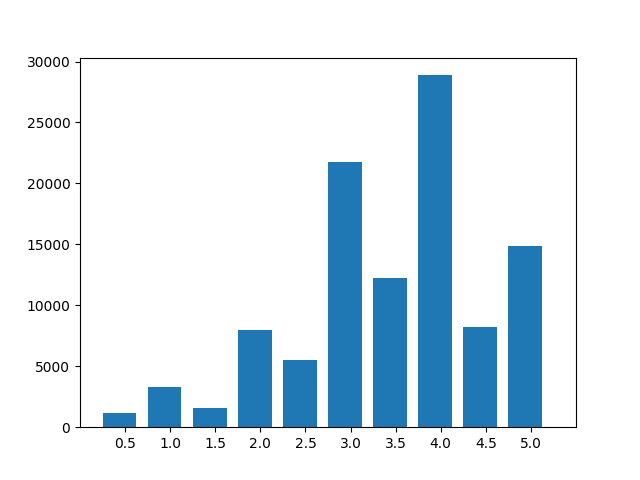
\includegraphics[scale=0.6]{small}
\caption{\emph{small} Movielens dataset ratings distribution}
\end{figure}

\begin{table}[H]
\centering
\begin{tabular}{l|r}
number of users N&  6040 \\ 
number of items M& 3706 \\
average rating & 3.58156 \\
standard deviation & 1.1171 \\
\end{tabular}
\caption{\emph{1M} Movielens dataset statistics}
\end{table}

\begin{figure}[H]
\centering
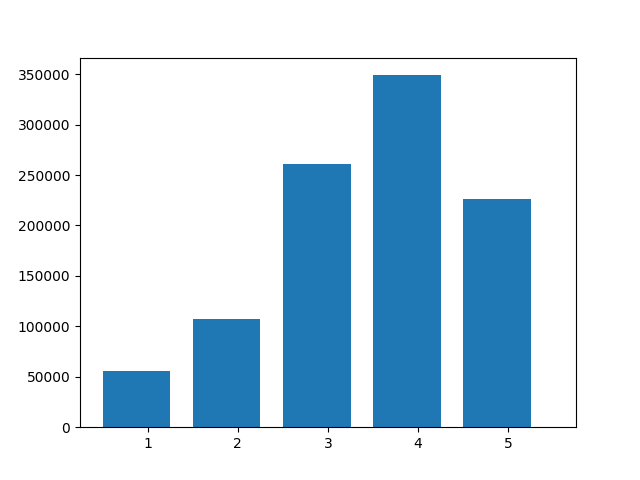
\includegraphics[scale=0.6]{1m}
\caption{\emph{1M} Movielens dataset ratings distribution}
\end{figure}

